\section{Experiments}
We conduct experiments on two ultra-fine entity typing datasets, {\bf \textsc{UFET}} (English) and {\bf \textsc{CFET}} (Chinese). Their data statistics are shown in Table \ref{tab:stat}. We mainly focus on and report the macro-averaged recall at the recall and expand stage, and concern mainly on the macro-$F1$ of the final prediction at the filter stage. We also evaluate the {\bf \textsc{\name}} models on the fine-grained (130 types) and coarse-grained (9 types) settings of entity typing without the recall and expand stage.
\subsection{UFET and CFET}
\subsubsection{Recall Stage}
\label{sec:recall}
We compare the recall@$K$ on the test sets of {\bf \textsc{UFET}} and {\bf\textsc{CFET}} between the trained MLC model (introduced in \ref{sec:mlc}) and a traditional BM25 model \cite{bm25} in Figure \ref{fig:recall}. The MLC model uses the RoBERTa-large as backbone and is tuned based on the recall@$128$ on the development set. We use AdamW optimizer with a learning rate of $2\times10^{-5}$. Results show that MLC is a strong recall model, it consistently has better recall compared to BM25 on both {\bf\textsc{UFET}} and {\bf\textsc{CFET}} dataset, and the recall@$128$ reaches over $85\%$ on {\bf \textsc{UFET}}, and over $94\%$ on {\bf \textsc{CFET}}.

\begin{figure}[t]
     \centering
     \begin{subfigure}[h]{0.5\textwidth}
         \centering
         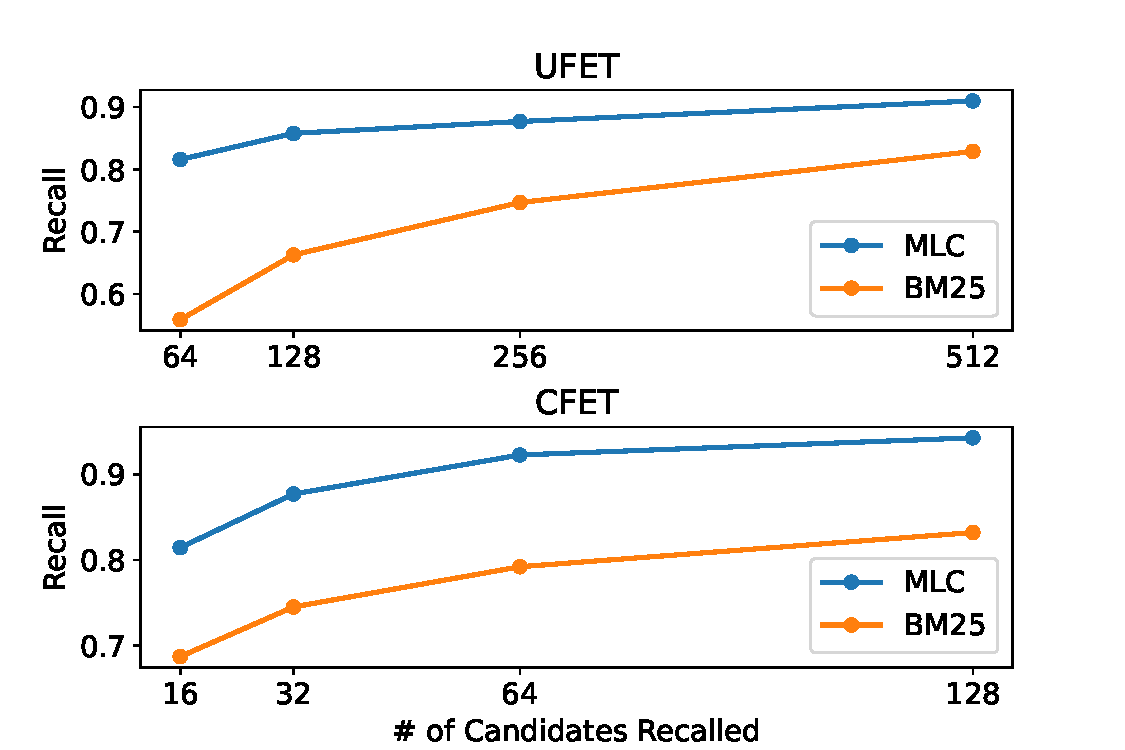
\includegraphics[width=\textwidth]{src/img/recall_compare_bm25.pdf}
         \label{fig:mb2}
     \end{subfigure}   
 \caption{Recall@$K$ of MLC and BM25.}
 \label{fig:recall}
\end{figure}

\subsection{Expand Stage}
\label{sec:expand}
In Table \ref{tab:expand}, we evaluate the F1 scores of all candidates expanded by exact match, and top-$10$ candidates expanded by the MLM using Bert-large. We also demonstrate the improvement of recall by using candidate expansion in Figure \ref{fig:expand_improvement}. On {\bf \textsc{UFET}} dataset, expanding around $32$ additional candidates based on $112$ MLC candidates results in $2\%$ higher recall compared to recalling all $128$ candidates by MLC. The recall of $128$ candidates after the expansion is comparable to the recall of $180$ candidates recalled from MLC. Similarly, expanding $10$ candidates is comparable to additionally recalling $80$ candidates using MLC.
In our experiments, we replace the last $48$ candidates recalled by MLC with the candidates recalled by MLM and Exact match for {\bf \textsc{UFET}} and $10$ for {\bf \textsc{CFET}}. We found the expand stage has a positive effect on the final performance of {\bf \textsc{\name}}s, and helps them reach SOTA performance (analyze in Sec. \ref{sec:analyze}).


\begin{table}[t]
\centering
\scalebox{0.75}{
\begin{tabular}{cccccc} 
\toprule
{\bf \textsc{Dataset}} & {\bf \textsc{Expand}} &   {\bf \textsc{P}}  & {\bf \textsc{R}}  &  {\bf \textsc{F1}} & \small{Avg \# Expanded}  \\ \midrule
\multirow{2}{*}{\bf \textsc{UFET}} & {\bf \textsc{Match}}      & 11.2   & 11.3     & 9.8    & 5.23     \\
      & {\bf \textsc{MLM}}  &  8.5     &   17.1   &  10.7  &    10    \\ \midrule
\multirow{2}{*}{\bf \textsc{CFET}} & {\bf \textsc{Match}}   &  11.4  &  14.5  & 11.2   & 4.57    \\
 & {\bf \textsc{MLM}}  & 21.3   &  19.5  & 17.7    & 10    \\ \midrule
\end{tabular}}
\caption{Evaluation of the recalled candidates.}
\label{tab:expand}
\end{table}
\begin{figure}[t]
     \centering
     \begin{subfigure}[h]{0.45\textwidth}
         \centering
         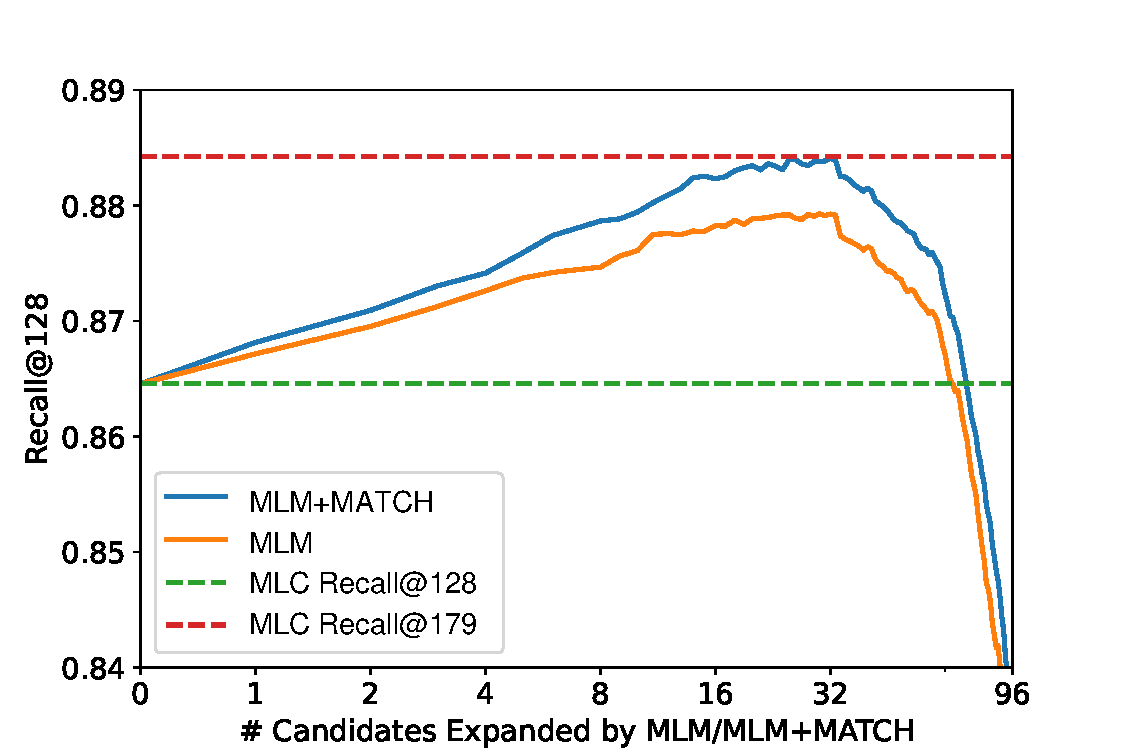
\includegraphics[width=\textwidth]{src/img/recall_ufet.pdf}
         \caption{Recall@$128$ on {\bf \textsc{UFET}} by including different number of expanded candidates. }
         \label{fig:c1}
     \end{subfigure}
     \vfill
     \begin{subfigure}[h]{0.45\textwidth}
         \centering
         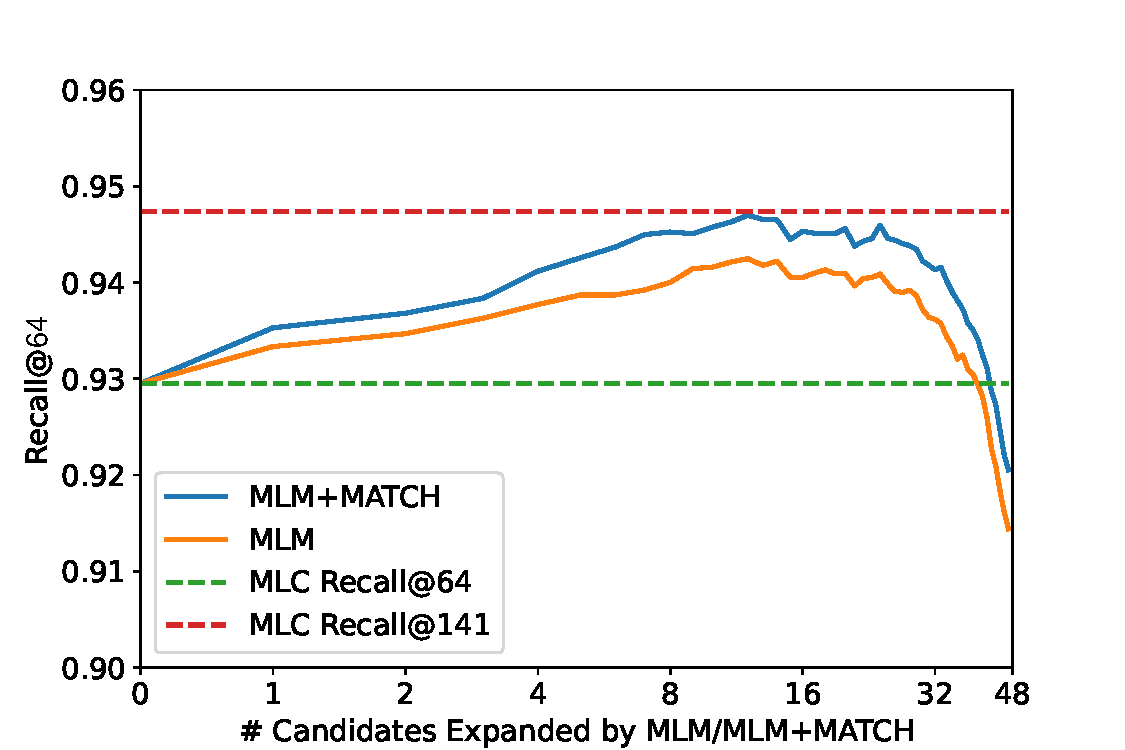
\includegraphics[width=\textwidth]{src/img/recall_cfet.pdf}
         \caption{Recall@$64$ on {\bf \textsc{CFET}} by including different number of expanded candidates.}
         \label{fig:c2}
     \end{subfigure}
\caption{Demonstration of the effect of expand stage. $x$-axis represents the number of candidates expanded by MLM/MLM+MATCH among these $128$ candidates. }
\label{fig:expand_improvement}
\end{figure}
\label{sec:exp_expand}
\subsection{Filter Stage and Final Results.}
\begin{table}[h!]
\centering
\scalebox{0.73}{
\renewcommand{\arraystretch}{1}
\begin{tabular}{cllll} \toprule
\multicolumn{2}{l}{\bf \textit{Base Models on UFET} }     & \bf \textsc{P}    & \bf \textsc{R}   & \bf \textsc{F1}  \\ \midrule
\multicolumn{5}{l}{\emph{MLC-like models}}        \\
\color{blue} \bf \texttt{B}& {\bf \textsc{Box4Types}}\cite{box4types}  & 52.8 & 38.8 & 44.8  \\
\color{blue}\bf \texttt{B}& {\bf \textsc{LDET}}$^\dagger$  \cite{onoe-durrett-2019-learning}          & 51.5 & 33.0 & 40.1 \\ 
\color{blue}\bf \texttt{B}& {\bf \textsc{MLMET}}$^\dagger$   {\cite{mlmet}}   & 53.6 & 45.3 & 49.1  \\
\color{blue}\bf \texttt{B}& {\bf \textsc{PL}}  \cite{ding2021prompt}   & 57.8 & 40.7 & 47.7 \\
\color{blue}\bf \texttt{B}& {\bf \textsc{DFET}}    \cite{dfet}      & 55.6 & 44.7 & 49.5 \\
\color{blue}\bf \texttt{B}& {\bf \textsc{MLC}} (reimplemented by us) & 46.5 & 34.9 & 39.9 \\ 
\color{red}\bf \texttt{R}& {\bf \textsc{MLC}} (reimplemented by us) & 42.2 & 44.9 & 43.5 \\ \hline 
\multicolumn{5}{l}{\emph{Seq2seq based models}}      \\
\color{blue}\bf \texttt{B} & {\bf \textsc{LRN} }  {\cite{liu-etal-2021-fine}}              & 54.5 & 38.9 & 45.4  \\\hline
\multicolumn{5}{l}{\emph{Filter models under our recall-expand-filter paradigm}}      \\
\color{blue}\bf \texttt{B} & {\bf \textsc{Vanilla CE}$_{128}$}   & 47.2 & 48.5 & 47.8 \\ 
\color{blue}\bf \texttt{B} & {\bf \textsc{\name-S$_{128}$}} (Ours)  & 53.2 & 48.3 & {\bf 50.6} \\ 
\color{blue}\bf \texttt{B} & {\bf \textsc{\name-S$_{128}$ w/o C2C}}   (Ours)   & 52.3 & 48.3 & 50.2 \\ 
\color{blue}\bf \texttt{B} & {\bf \textsc{\name-B$_{128}$}} (Ours)    & 49.9 & 50.0 & 49.9 \\ 
\color{blue}\bf \texttt{B} & {\bf \textsc{\name-B$_{128}$ w/o C2C}} (Ours)     & 49.9 & 48.2 & 49.0 \\ \hline
\color{red}\bf \texttt{R} & {\bf \textsc{Vanilla CE}$_{128}$}   & 49.6 & 49.0 & 49.3 \\ 
\color{red}\bf \texttt{R} & {\bf \textsc{\name-S$_{128}$}} (Ours)  & 53.3 & 47.3 & 50.1 \\ 
\color{red}\bf \texttt{R} & {\bf \textsc{\name-S$_{128}$ w/o C2C}}   (Ours)  & 53.2 & 46.6 & 49.7 \\ 
\color{red}\bf \texttt{R} & {\bf \textsc{\name-B$_{128}$}} (Ours)  & 52.5 & 47.9 & 50.1 \\ 
\color{red}\bf \texttt{R} & {\bf \textsc{\name-B$_{128}$ w/o C2C}} (Ours)     & 52.7 & 46.4 & 49.3 \\ \hline
\midrule
\multicolumn{2}{l}{\bf \textit{Large Models on UFET} }     & \bf \textsc{P}    & \bf \textsc{R}   & \bf \textsc{F1}  \\ \midrule
\multicolumn{5}{l}{\emph{MLC-like models}}        \\
\color{red}\bf \texttt{R} & {\bf \textsc{MLC}}  \cite{npcrf}               & 47.8 & 40.4 & 43.8  \\
\color{red}\bf \texttt{R} & {\bf \textsc{MLC-NPCRF}} \cite{npcrf}             & 48.7 & 45.5 & 47.0  \\
\color{red}\bf \texttt{R} & {\bf \textsc{MLC-GCN}} \cite{xiong-etal-2019-imposing}     & 51.2 & 41.0 & 45.5 \\
\color{blue}\bf \texttt{B} & {\bf \textsc{PL}}  \cite{ding2021prompt}       & 59.3 & 42.6 & 49.6  \\
\color{blue}\bf \texttt{B} & {\bf \textsc{PL-NPCRF}}  \cite{npcrf}  & 55.3 & 46.7 & {50.6}\\ \hline
\multicolumn{4}{l}{\emph{Cross-encoder based models and {\bf \textsc{\name}}s}}      \\
\color{red}\bf \texttt{R} & {\bf \textsc{LITE+L}}  \cite{lite}             & 48.7 & 45.8 & 47.2  \\
\color{teal}\bf \texttt{RM} & {\bf \textsc{LITE+NLI+L}} \cite{lite} & 52.4 & 48.9 & {50.6} \\ \hline
\multicolumn{4}{l}{\emph{Filter models under our recall-expand-filter paradigm}}   \\ 
\color{blue}\bf \texttt{B} & {\bf \textsc{Vanilla CE$_{128}$}}   & 50.3 & 49.6 & 49.9 \\ 
\color{blue}\bf \texttt{B} & {\bf \textsc{\name-S$_{128}$}}  (Ours)   & 52.5 & 49.1 & 50.8 \\ 
\color{blue}\bf \texttt{B} & {\bf \textsc{\name-S$_{128}$ w/o C2C}}   (Ours)   & 54.1 & 47.1 & 50.4 \\ 
\color{blue}\bf \texttt{B} & {\bf \textsc{\name-B$_{128}$}} (Ours)    & 54.0 & 48.6 & 51.2 \\ 
\color{blue}\bf \texttt{B} & {\bf \textsc{\name-B$_{128}$ w/o C2C}} (Ours)     & 52.8 & 48.3 & 50.4 \\ \hline
\color{red}\bf \texttt{R} & {\bf \textsc{Vanilla CE$_{128}$}}   & 54.5 & 49.3 & 51.8 \\ 
\color{red}\bf \texttt{R} & {\bf \textsc{\name-S$_{128}$}}  (Ours)   & 50.8 & 49.8  &  50.3 \\ 
\color{red}\bf \texttt{R} & {\bf \textsc{\name-S$_{128}$ w/o C2C}}   (Ours)   & 51.5 & 48.8 & 50.1 \\ 
\color{red}\bf \texttt{R} & {\bf \textsc{\name-B$_{128}$}} (Ours)    & 51.9 & 50.8 & 51.4 \\ 
\color{red}\bf \texttt{R} & {\bf \textsc{\name-B$_{128}$ w/o C2C}} (Ours)     & 51.6 & 51.6 & 51.6 \\ \hline
\color{teal}\bf \texttt{RM} & {\bf \textsc{\name-B$_{128}$ w/o C2C}} (Ours) & 56.3 & 48.5 & {\bf 52.1} \\ \hline
\midrule
\end{tabular}}
\caption{Macro-averaged UFET result. {\bf \textsc{LITE+L}} is LITE without NLI pretraining, {\bf \textsc{LITE+L+NLI}} is the full LITE model. Methods marked by $\dagger$ utilize either distantly supervised or augmented data for training. {\bf \textsc{\name-S$_{128}$}} denotes we use $128$ candidates recalled and expanded from the first two stages.}
\label{tab:ufet}
\end{table}
\begin{table}[t]
\centering
\scalebox{0.75}{
\renewcommand{\arraystretch}{1}
\begin{tabular}{cllll} \toprule
\multicolumn{2}{l}{\bf \textit{Models on CFET} }     & \bf \textsc{P}    & \bf \textsc{R}   & \bf \textsc{F1}  \\ \midrule
\multicolumn{5}{l}{\emph{MLC-like models}}        \\
\color{purple}\bf \texttt{N}& {\bf \textsc{MLC}} & 55.8 & 58.6 & 57.1 \\  
\color{purple}\bf \texttt{N}& {\bf \textsc{MLC-NPCRF}} \cite{npcrf}     & 57.0 & 60.5 & 58.7 \\ 
\color{purple}\bf \texttt{N}& {\bf \textsc{MLC-GCN}} \cite{xiong-etal-2019-imposing}   & 51.6 & 63.2 & 56.8 \\ 
\color{brown}\bf \texttt{C}& {\bf \textsc{MLC}} & 54.0 & 59.5 & 56.6 \\  
\color{brown}\bf \texttt{C}& {\bf \textsc{MLC-NPCRF}} \cite{npcrf}   & 54.0 & 61.6 & 57.3 \\  
\color{brown}\bf \texttt{C}& {\bf \textsc{MLC-GCN}} \cite{xiong-etal-2019-imposing} & 56.4 & 58.6 & 57.5 \\ \midrule 
\multicolumn{5}{l}{\emph{Filter models under our recall-expand-filter paradigm}}      \\
\color{purple}\bf \texttt{N} & {\bf \textsc{Vanilla CE}}   & 57.6 & 64.3 & 60.7 \\ 
\color{brown}\bf \texttt{C} & {\bf \textsc{Vanilla CE}}   & 54.0 & 63.3 & 58.3 \\  \hline
\color{purple}\bf \texttt{N} & {\bf \textsc{\name-S$_{64}$}} (Ours)  & 58.4 & 62.1 & 60.2 \\ 
\color{purple}\bf \texttt{N} & {\bf \textsc{\name-S$_{64}$ w/o C2C}}   (Ours)   & 59.1 & 61.5 & 60.3 \\ 
\color{purple}\bf \texttt{N} & {\bf \textsc{\name-B$_{64}$}} (Ours)    & 56.7 & 66.1 & 61.1 \\ 
\color{purple}\bf \texttt{N} & {\bf \textsc{\name-B$_{64}$ w/o C2C}} (Ours)     & 58.8 & 64.1 & 61.4 \\ \hline
\color{brown}\bf \texttt{C} & {\bf \textsc{\name-S$_{64}$}} (Ours)  & 55.5 & 62.6 & 58.8 \\ 
\color{brown}\bf \texttt{C} & {\bf \textsc{\name-S$_{64}$ w/o C2C}}   (Ours)   & 54.0 & 63.4 & 58.3 \\ 
\color{brown}\bf \texttt{C} & {\bf \textsc{\name-B$_{64}$}} (Ours)    & 55.0 & 63.5 & 59.0 \\ 
\color{brown}\bf \texttt{C} & {\bf \textsc{\name-B$_{64}$ w/o C2C}} (Ours)     & 57.3 & 61.3 & 59.3 \\ \hline
\midrule
\end{tabular}}
\caption{Macro-averaged CFET result.}
\label{tab:cfet}
\end{table}

In this section, we report the performance of {\bf \textsc{MCCE}} variants as the filter models and compare them with various strong baselines that we will introduce later. We also compare the inference speed of different models in this section. For filter models, we treat the number of candidates $K$ recalled and expanded by the first two stages as hyper-parameters, and tune it on the development set. We found the choice of PLM backbones has a non-negligible effect on the performance, and the PLM backbone of previous methods varies. Therefore for fairer comparisons to baselines, we conduct experiments of {\bf \textsc{\name}} using different backbone PLMs for our {\bf \textsc{\name}} models and report the results. For all {\bf \textsc{\name}} models, we use AdamW optimizer with a learning rate tuned between $5\times 10^{-6}$ and $2\times 10^{-5}$. The batch size we use is $4$ and we train the models for at most $50$ epochs with early stopping. {\bf \textsc{UFET}} also provides a large dataset obtained from distant supervision such as entity linking, we do not use it and only train and evaluate our models on human-labeled data.
\paragraph{Baselines}
The {\bf \textsc{MLC}} model we used for the recall stage and the cross-encoder ({\bf \textsc{CE}}) we introduced in Sec. \ref{sec:vanilla_ce} are natural baselines. We also compare our methods with recent PLM-based methods. {\bf \textsc{LDET} }\cite{onoe-durrett-2019-learning} is an MLC with Bert-base-uncased and ELMo \cite{elmo} trained on 727k examples automatically denoised from the distantly labeled UFET. {\bf \textsc{GCN} }\cite{xiong-etal-2019-imposing} uses GCN to model type correlations and obtain type embeddings. Types are scored by dot-product of mention and type embeddings. The original paper uses BiLSTM as the mention encoder and we use the results re-implemented by \citet{npcrf} using RoBERTa-large. {\bf \textsc{Box4Type} }\cite{box4types} uses Bert-large as the backbone and uses box embedding to encode mentions and types for training and inference. {\bf \textsc{LRN} }\cite{liu-etal-2021-fine} use Bert-base as the encoder and an LSTM decoder to generate types in a seq2seq manner. {\bf \textsc{MLMET} }\cite{mlmet} is a {\bf \textsc{MLC}} with Bert-base, but first pretrained by the distantly-labeled data augmented by masked word prediction, then finetuned and self-trained on the 2k human-annotated data. {\bf \textsc{PL}} \cite{ding2021prompt} uses prompt learning for entity typing. {\bf \textsc{DFET} }\cite{dfet} uses {\bf \textsc{PL}} as backbone and is a multi-round automatic denoising method for 2k labeled data. {\bf \textsc{LITE} }\cite{lite} is the previous SOTA system that formulates entity typing as textual inference. {\bf \textsc{LITE}} uses RoBERTa-large-MNLI as the backbone, and is a cross-encoder (introduced in Sec. \ref{sec:vanilla_ce}) with designed templates and a hierarchical loss. \citet{npcrf} proposes {\bf \textsc{NPCRF}} to enhance backbones such as {\bf \textsc{PL}} and {\bf \textsc{MLC}} by modeling type correlations, and reach performance comparable to {\bf \textsc{LITE}}.

\paragraph{Naming Conventions}
Let {\bf \textsc{\name-S}} be the {\bf \textsc{\name}} model that treats candidates as sub-tokens, and {\bf \textsc{\name-B}} be the model representing candidates as fixed-size blocks. The {\bf \textsc{\name}} model without {\bf \textsc{C2C}} attention (mentioned in Sec. \ref{sec:attn}) is denoted as {\bf \textsc{\name-B} w/o C2C}. For PLM backbones used in {\bf \textsc{UFET}}, we use {\color{blue} \bf \texttt{B}}, {\color{red} \bf \texttt{R}}, {\color{teal} \bf \texttt{RM}} to denote BERT-base-cased \cite{bert}, RoBERTa \cite{liu2019roberta}, and RoBERTa-MNLI \cite{liu2019roberta} respectively. For {\bf \textsc{CFET}}, we adopt two widely-used Chinese PLM, BERT-base-Chinese and NeZha-base-Chinese, and denote them as {\color{brown} \bf \texttt{C}} and {\color{purple} \bf \texttt{N}} respectively. 

\paragraph{UFET Results} We show the results of {\bf \textsc{UFET}} dataset in Table \ref{tab:ufet}. The results show that: (1) The recall-expand-filter paradigm is effective. Filter models outperform all baselines without the paradigm by a large margin. The vanilla CE under our paradigm reaches $51.8$ F1 compared to more complexed CE {\bf \textsc{LITE}} with $50.6$ F1 (2) {\bf \textsc{\name}} models reach SOTA performances. {\bf \textsc{\name-S$_{128}$}} with BERT-base performs best and reaches {\bf 50.6} F1 score, which is comparable to previous SOTA performance of large models such as {\bf \textsc{LITE+NLI+L}} and {\bf \textsc{PL+NPCRF}}. Among large models, {\bf \textsc{\name-B$_{128}$ w/o C2C}} also reaches SOTA performance with {\bf 52.1} F1 score. (3) {\bf \textsc{C2C}} attention is not necessary on large models, but is useful in base models. (4) Large models can utilize type semantics better. We found {\bf \textsc{\name-B}} outperforms {\bf \textsc{\name-S}} on large models, but underperforms {\bf \textsc{\name-S}} on base models. (5) Backbone PLM matters. We found the performance of {\bf \textsc{Vannila CE}} under our paradigm is largely affected by the PLM it used. It reaches $47.8$ F1 with BERT-base and $51.8$ F1 with RoBERTa-large. For {\bf \textsc{\name}} models, we found {\bf \textsc{\name}} performs better than {\bf \textsc{\name-B}} with BERT, and worse than {\bf \textsc{\name-B}} with RoBERTa. 

\begin{table*}[t]
\centering
\scalebox{0.9}{
\begin{tabular}{lllcc} \toprule
\bf \textsc{Model}  & \bf \textsc{\# FP} & \bf \textsc{Attn} & \bf \textsc{sents/sec} & \bf \textsc{F1} \\ \midrule
{\bf \textsc{MLC}} & \small{$1$}  & \small{$L_S^2D$} & 58.8 & 43.8\\
{\bf \textsc{LITE+NLI+L (CE)}}  & \small{$N$}  & \small{$L_S^2D$} & 0.02 & 50.6\\ \midrule \hline
\multicolumn{5}{l}{\emph{filter stage inference speed.}}  \\
{\bf \textsc{Vanilla CE$_{128}$}}  & \small{$128$}  & \small{$L_S^2D$} & 1.64 & 51.8 \\ 
{\bf \textsc{\name-S$_{128}$}}  & \small{$1$}  & \small{$(L_S+128)^2D$} & 60.8 & 50.1 \\ 
{\bf \textsc{\name-B$_{128}$}}  & \small{$1$}  & \small{$(L_S+128B)^2D$} & 22.3 & 51.4\\ 
{\bf \textsc{\name-B$_{128}$ w/o C2C}}  & \small{$1$}  & \small{$(L_S^2+256L_S B + 128 B^2)D$} & 25.2 & {\bf 52.1}\\ \bottomrule
\end{tabular}}
\caption{Inference speed comparison of models. {\bf \textsc{\# FP}} means the number of PLM forward passes required by a single inference. {\bf \textsc{ATTN}} column lists the theoretical attention complexity.  We also report the practical inference speed {\bf \textsc{sents/sec}} and the {\bf \textsc{F1}} scores on {\bf \textsc{UFET}} with RoBERTa-large architecture.}
\label{tab:speed}
\end{table*}

\begin{table}[t]
\centering
\scalebox{0.85}{
\renewcommand{\arraystretch}{1}
\begin{tabular}{cllll} \toprule
\multicolumn{2}{l}{\bf \textit{Models} }     & \bf \textsc{P}    & \bf \textsc{R}   & \bf \textsc{F1}  \\ \midrule
\multicolumn{5}{l}{\emph{coarse (9 types) Open Entity}}        \\ \hline
\color{red}\bf \texttt{R} & {\bf \textsc{MLC}}   & 76.8 & 78.5 & 77.6 \\ 
\color{red}\bf \texttt{R} & {\bf \textsc{Vanilla CE$_{9}$}}   & 82.3 & 81.0 & 81.6 \\ 
\color{red}\bf \texttt{R} & {\bf \textsc{\name-S$_{9}$}}   & 77.0 & 87.7 & 82.0 \\ 
\color{red}\bf \texttt{R} & {\bf \textsc{\name-B$_{9}$ w/o C2C}}   & 77.2 & 85.4 & 81.1 \\ \hline
\multicolumn{5}{l}{\emph{fine (130 types)}}        \\ \hline
\color{red}\bf \texttt{R} & {\bf \textsc{MLC}}   & 70.4 & 63.7 & 66.9  \\ 
\color{red}\bf \texttt{R} & {\bf \textsc{Vanilla CE}$_{130}$}   & 67.9 & 66.4 & 67.1 \\ 
\color{red}\bf \texttt{R} & {\bf \textsc{\name-S$_{130}$}}   & 65.8 & 71.8 & 68.7 \\ 
\color{red}\bf \texttt{R} & {\bf \textsc{\name-B$_{130}$ w/o C2C}}   & 64.1 & 70.5 & 67.1 \\ \hline
\midrule
\end{tabular}}
\caption{Micro-averaged results on UFET fine and coarse.}
\label{tab:ufet-coarse-fine}
\end{table}

\paragraph{CFET Results} We conduct experiments on {\bf \textsc{CFET}} and compare {\bf \textsc{\name}} models with several strong baselines:  {\bf \textsc{NPCRF}} and {\bf \textsc{GCN}} with MLC-like architecture, and {\bf \textsc{Vanilla CE}} under out paradigm which is proved to be better than {\bf \textsc{LITE}} on {\bf \textsc{UFET}}. The results are shown in Table \ref{tab:cfet}. Similar to results in {\bf \textsc{UFET}}, filter models under our paradigm significantly outperform MLC-like baselines, $+2.0$ F1 for Nezha-base and $+1.8$ F1 for BERT-base-Chinese. In {\bf \textsc{CFET}}, {\bf \textsc{\name}-B} is significantly better than {\bf \textsc{\name}-S}, on both Nezha-base and BERT-base-Chinese, indicating the importance of type semantics in Chinese language. We also find that {\bf \textsc{\name} w/o C2C} is generally better than  {\bf \textsc{\name} w/ C2C}, it is possibly because the C2C attention distracts the candidates from attending to mention and contexts.
\paragraph{Speed Comparison} Table \ref{tab:speed} shows the theoretical inference complexity (number of PLM forward passes, and attention complexity), and practical inference speed (number of sentences inferred per second) of different models. We conduct the speed test using NVIDIA TITAN RTX for all models, and the inference batch size is 4.
At the filter stage, the inference speed of {\bf \textsc{\name-S}} is on par with {\bf \textsc{MLC}} (even slightly faster because we don't need to score all types), and is about 40 times faster than {\bf \textsc{Vannila CE}} and thousands of times faster than {\bf \textsc{LITE}}. {\bf \textsc{\name-B w/o C2C}} is not significantly faster than {\bf \textsc{\name-B}} as expected. It's possibly because the computation related to the block attention is not fully optimized by existing deep learning frameworks. The speed advantage of {\bf \textsc{\name-B w/o C2C}} over {\bf \textsc{\name-B}} will be greater with more candidates.


\subsection{Fine-grained and Coarse-grained Entity Typing}
We also conduct experiments on Fine-grained (130-class) and Coarse-grained (9-class, also known as ``Open Entity'') entity typing, and the results are shown in Table \ref{tab:ufet-coarse-fine}. As the type candidate set is much smaller in these settings, we skip the recall and expand stages and directly run the filter models and compare them to baselines. Results show that both {\bf \textsc{\name}-S} and {\bf \textsc{\name}-B} are still better than {\bf \textsc{MLC}} and {\bf \textsc{Vanilla CE}}, and {\bf \textsc{\name}-S} is better than {\bf \textsc{\name}-B} on coarser-grained cases possibly because the coarser-grained types are simpler in surface-forms and {\bf \textsc{\name}-S} will not lose many type semantics.




